\documentclass[a4paper]{article}

\usepackage[utf8]{inputenc}
\usepackage[serbian]{babel}

\usepackage{tikz}
\usepackage{tcolorbox}
\usepackage{amsmath}
\usepackage{amsthm}
\usepackage{amsfonts}	
\usepackage{float}
\usepackage{listings}
\usepackage{fancyhdr}


\begin{document}
    \begin{titlepage}
    \begin{tabular}{ l  c   r  }
        
\includegraphics[height=0.1\textwidth, width=0.1\textwidth]{img/uns.png} &
        \begin{tabular}{c}
            \large\textbf{UNIVERZITET U NOVOM SADU} \\
            \large\textbf{FAKULTET TEHNIČKIH NAUKA}  \\
        \end{tabular}
        
\includegraphics[height=0.1\textwidth, width=0.1\textwidth]{img/ftn-logo.jpg}
    \end{tabular}
    \vspace*{1cm}
    \begin{flushleft}
        UNIVERZITET U NOVOM SADU \\
        FAKULTET TEHNIČKIH NAUKA \\
        NOVI SAD \\
    \end{flushleft}
    \vspace*{2cm}
    \begin{center}
        \LARGE\textbf{Aplikacija za praćenje zbrinjavanja životinja}
    \end{center}
    \vspace*{0.25cm}
    \begin{flushleft}
        \begin{tabular}{l l l}
            Kandidati:& Lazar Nagulov & SV61/2022\\
                      & Filip Tot & SV14/2022 \\
                      & Ilija Jordanovski & SV73/2022 \\
                      & Vuk Vićentić & SV45/2022 \\
            & \\
            Predmet:& Specifikacija i modeliranje softvera \\
        \end{tabular}
    \end{flushleft}
    \vfill
    \begin{center}
        Novi Sad, jul, 2024.
    \end{center}
\end{titlepage}
    \pagestyle{fancy}
    
\rhead{SADRŽAJ}
\lhead{}
\pagenumbering{Roman}
\tableofcontents
\newpage

\rhead{SPISAK SLIKA}
\listoffigures
\newpage

\rhead{SPISAK TABELA}
\listoftables
    \pagenumbering{arabic}

    \rhead{Funkcionalni zahtevi}
    \section{Funkcionalni zahtevi}
    \par Aplikacija za praćenje zbrinjavanja životinja omogućava olakšano pronalaženje novog vlasnika za životinje. 
    \par Na osnovu dijagrama slučajeva korišćenja [Slika \ref{fig:use-case}] primećujemo da postoje četiri uloge u aplikaciji: neregistrovani korisnik (osoba), korisnik, volonter i administrator. U nastavku se nalazi 
    opis funkcionalnosti za svaku od uloga.
    \begin{enumerate}
        \item \textbf{Neregistrovani korisnik (osoba)} - mogućnost registracije unošenjem imena, prezimena, adrese, korisničkog imena i šifre;
        prijavljivanja na sistem unosom korisničkog imena i šifre, kao pregled odobrenih objava.
        \item \textbf{Korisnik} - poseduje sve mogućnosti kao i \textit{neregistrovani korisnik}. Dodatno može da kreira objavu (koja mora biti prihvaćena od strane
        \textit{volontera}) birajući već postojeći tip životinje, komentariše i lajkuje odobrene objave. Za svaku odobrenu objavu, ima mogućnost da pošalje zahtev za udomljavanje ili 
        privremeni smeštaj. On uvek ima uvid u sve svoje zahteve, gde po mogućnosti može da odustane od njih. Ukoliko se zahtev odobri od strane \textit{volontera}, stanje objave se menja, 
        ali i dalje se prikazuje korisnicima. U svakom trenutku nakon udomljavanja ili obezbeđenog privremenog smeštaja, \textit{korisnik} može da oceni životinju sa brojem i komentarom, 
        kao i da je vrati nazad, ukoliko nije zadovoljan. Korisniku se takođe nudi mogućnost doniranja novca za pomoć udruženju.
        \item \textbf{Volonter} - poseduje sve mogućnosti kao i \textit{korisnik}, stim da je njegova objava automatski prihvaćena. Da bi \textit{korisnik} postao \textit{volonter}, on mora
        da bude izglasan od strane drugih \textit{volontera} (prvog volontera dodaje \textit{administrator}). On je zadužen za prihvatanje objava od strane korisnika i sakrivanje već 
        prihvaćenih objava. Ima pristup listi svih ponuda o udomljavanju i obezbeđivanju privremenog smeštaja, gde može da prihvati ili odbije ponude. Dodatno je zadužen za unos uplate od 
        strane korisnika i raspoređivanje sredstava po životinjama. Takođe može da dodaje, briše i menja podatke o vrsti životinja. 
        \item \textbf{Administrator} - poseduje sve mogućnosti kao i \textit{korisnik}. Dodatno dodaje, briše i menja informacije o udruženju i dodaje prvog \textit{volontera}.
    \end{enumerate} 
    \begin{figure}
        \centering
        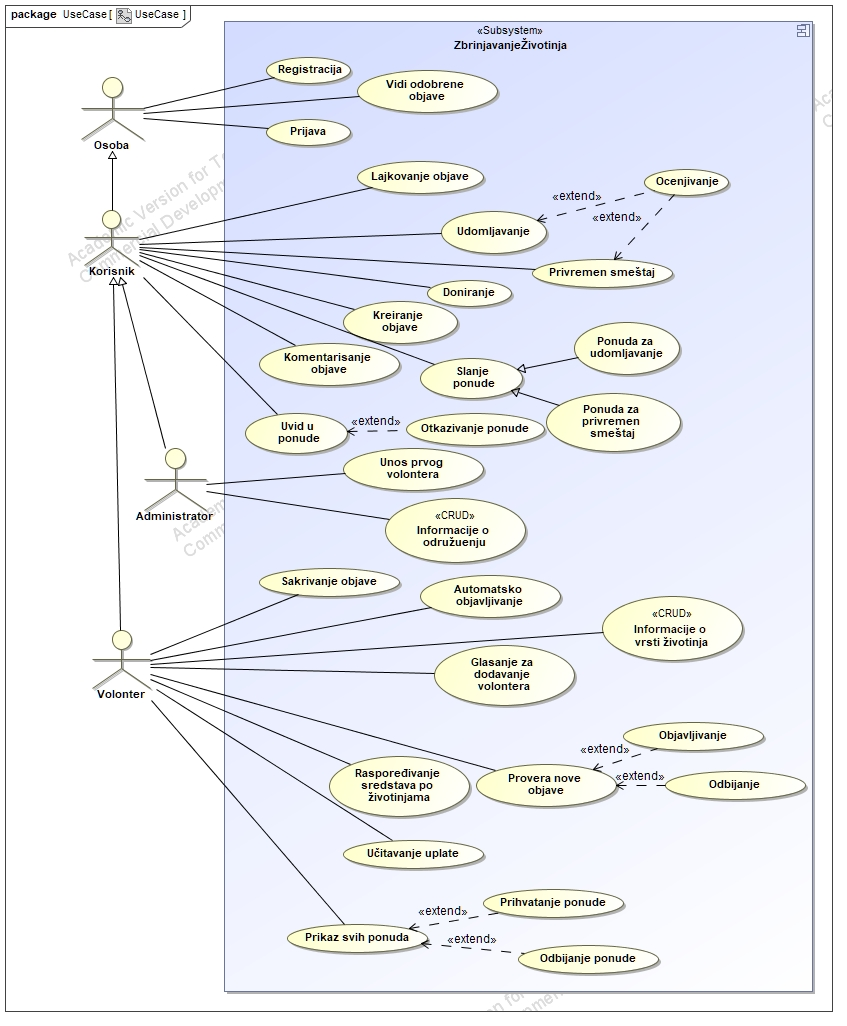
\includegraphics[width=\textwidth]{img/use-case.jpg}
        \caption{Dijagram slučajeva korišćenja}
        \label{fig:use-case}
    \end{figure}

\end{document}
